\documentclass[letterpaper]{article}
\title{CSE 546 Machine Learning, Autumn 2013 \\ Homework 4}
\date{Shrainik Jain, 1323338}

\usepackage[margin=1in]{geometry}

\usepackage{amsmath}
\usepackage{amssymb}

%\usepackage{algpseudocode}
%\usepackage{algorithmicx}
\usepackage{alltt}

\usepackage[normalem]{ulem}
\usepackage{float}
\usepackage{enumitem}
\usepackage{graphicx}
\usepackage{listings}

\setlist{noitemsep}

\newcommand{\ind}{\hspace{1cm}} 
\newcommand{\m}[1]{\mathbf{#1}}
\newcommand{\x}{\m{x}}
\newcommand{\bigC}{\mathbf{C}}
\newcommand{\bigX}{\mathbf{X}}
\newcommand{\bigI}{\mathbf{I}}

\begin{document}
\maketitle

\section{Learning Theory [30 points]}


\begin{enumerate}
\item For \[h \, : \, \{ 0, 1 \}^d \rightarrow \{ 0, 1 \} \] the feature space is of dimension d. Since the features are binary, they can take 2 values, i.e. 0 or 1. This means that there are $2^d$ feature vectors in feature space. For each of these feature vector the output can take the value 0 or 1, i.e. 2 values possible per feature vector. Hence, total number of functions which map feature vector space to output space \[|H| = 2^{2^d}\]
\item Chernoff bound to estimate error of union over a total of $|H|$ hypotheses is:
\begin{equation}
P(error_{true}(h) - error_{train}(h) > \epsilon) \leq |H|\exp^{-2N\epsilon^2}
\end{equation}
for this problem, we want this to be bounded by $\delta$: \\
$\Rightarrow |H|\exp^{-2N\epsilon^2} \leq \delta $\\
This gives,
\begin{equation}
N \geq \frac{ln(\frac{|H|}{\delta})}{2\epsilon^2} \Rightarrow N \geq \frac{ln(\frac{2^{2^d}}{\delta})}{2\epsilon^2}
\end{equation}

\item From part 2, we see that the bound on N is $O(ln(2^{2^d})) = O(2^d)$ which means that the number of points needed to be sure of having generalization error less than $\epsilon$ with a high probability $1 - \delta$ increases exponentially with the incerease in the number of features. In practice, exponential number of data points are not available, hence this bound is not very useful.\\
\item From the lecture slides on learning theory, we know that the upper bound on number of decision trees of depth k ($|H|$) is $2^{(2^k -  1)(1+log_2d) +1}$. (Slide 34, learning theory.)\\
Which becomes $2^{2^k}d^{2^k-1}$ and $k=2 \Rightarrow |H| = 16d^3$\\\\
Plugging in $|H|$ to equation 1 above, we get, \\
\begin{equation}
N \geq \frac{ln(\frac{16d^3}{\delta})}{2\epsilon^2}
\end{equation}
\item The bound we got earlier (in part 2) was $O(2^d)$, where as the newer bound is $O(ln(16d^3)) = O(ln(d)).$ \\
This means that by restricting the structure of the problem, i.e. by restricting the hypothesis space to have only decision trees of depth 2, we require O(ln(d)) number of data points to get the similar PAC bound (instead of exponential number of points as in part 2 where there was no restriction on hypothesis space). Also, for a fixed depth, the number of data points required for the same PAC bound, are no longer exponential in dimension d. Which is a big big advantage. 
\end{enumerate}

\section{PCA via Successive Deflation [35 points]}

\begin{enumerate}
\item 
We have:\\\\
 $\tilde \bigC = \frac{1}{n} \tilde \bigX \tilde \bigX^T = \frac{1}{n}((\bigI - v_1 v_1^T) \bigX((\bigI - v_1 v_1^T) \bigX)^{T})$ \\

(using the fact that $(AB)^T = B^TA^T$ and $(\bigI - v_1 v_1^T)$ is symmetric)\\\\
\begin{equation}
\tilde \bigC  = \frac{1}{n} (\bigI - v_1 v_1^T)XX^T(\bigI - v_1 v_1^T)
\end{equation}
\begin{equation}
\tilde \bigC  = \frac{1}{n} (XX^T - v_1 v_1^TXX^T -XX^Tv_1 v_1^T + v_1 v_1^TXX^Tv_1 v_1^T)
\end{equation}

We know that $XX^Tv_1 = n\lambda_1v_1 \Rightarrow (XX^Tv_1)^T = (n\lambda_1v_1)^T \Rightarrow v_1^TXX^T = n\lambda_1v_1^T$ \\
Plugging into equation 5 we get, 
\begin{equation}
\tilde \bigC  = \frac{1}{n} (XX^T -v_1n\lambda_1v_1^T -n\lambda_1v_1v_1^T + v_1n\lambda_1v_1^Tv_1v_1^T)
\end{equation}

Finally, since $v_1^Tv_1 = 1$
\begin{equation}
\tilde \bigC = \frac{1}{n}XX^T - \lambda_1v_1v_1^T \,\,\, ... Q.E.D.
\end{equation}

\item We have:
$\tilde \bigC v_j = (\frac{1}{n}XX^T - \lambda_1v_1v_1^T)v_j$\\\\
$= \frac{1}{n}(XX^Tv_j) - \lambda_1v_1v_1^Tv_j$ \\\\
$= \lambda_jv_j - \lambda_1v_1v_1^Tv_j$  (since $XX^Tv_j = n\lambda_jv_j$)\\ \\
$\Rightarrow \tilde \bigC v_j = \lambda_jv_j$ (since $v_1^Tv_j = 0$ for $j \neq 1$) \\ and\\ $ \tilde \bigC v_1 = \lambda_1v_1 - \lambda_1v_1v_1^Tv_1 = (\lambda_1 - \lambda_1)v_1 = 0 v_1 = 0$ for $j=1$\\\\
hence, for $j \neq 1$, $v_j$ is also a principle eigenvector of $\tilde \bigC$ with same eigenvalue $\lambda_j$. \textbf{Also, $v_1$ is an eigenvector of $\tilde \bigC$ with eigenvalue 0.}\\
\item Since $v_1, v_2, \ldots v_k$ are the first $k$ eigenvectors with largest eigenvalues of $\bigC$, i.e., the principal basis vectors, therefore
\begin{equation}
\lambda_1 \ge \lambda_2 \ge \ldots \ge \lambda_k
\end{equation}
From part 2, we know that for $\tilde \bigC$, $v_j$ are the principle eigenvectors with eigenvalues $(0,\lambda_2,\lambda_3, \ldots, \lambda_k)$. Therefore from equation 8 above, $\lambda_2$ is the largest eigenvalue of $\tilde \bigC$ (since $\lambda_1$ is not an eigenvalue of $\tilde \bigC$), hence $v_2$ is the first principle eigenvector.
\\
\item  Pseudocode for finding the first $K$ principal eigenvectors of $\bigC$:
\begin{lstlisting}
def findEigenVectors(C,K,f):
	list_Lambda = []
	list_v = []
	for i in range(K):
		lambda, v = f(C)
		C = C - lambda * v * v.Transpose
		list_Lambda.append(lambda)
		list_v.append(v)
	return list_v, list_Lambda
\end{lstlisting}
\end{enumerate}


\section{Programming Question (clustering with K-means) [35 points]}


\subsection{The Data}
No Questions in this part.

\subsection{The algorithm}
No Questions in this part.

\subsection{Within group sum of squares}
No Questions in this part.

\subsection{Mistake Rate}
No Questions in this part.

\subsection{Questions}

\begin{enumerate}
\item 
For $k=2$
\begin{itemize}
\item Sum of within group sum of squares $= 536477102.543$
\item Mistake Rate $= 0.52$
\end{itemize}
For $k=4$
\begin{itemize}
\item Sum of within group sum of squares $= 461110943.962$
\item Mistake Rate $= 0.243$
\end{itemize}
For $k=6$
\begin{itemize}
\item Sum of within group sum of squares $= 431349182.916$
\item Mistake Rate $= 0.18$
\end{itemize}
\item The number of iterations that k-means ran for $k = 6$: \textbf{8 iterations.}
\item Plot for the sum of within group sum of squares versus $k$ for
$k = 1, 2, 3, 4, 5, 6, 7, 8, 9, 10$. Centers chosen randomly:\\
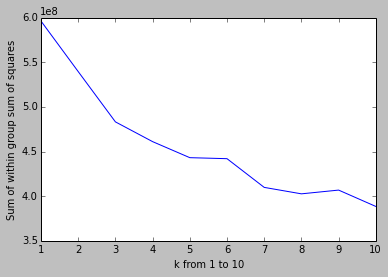
\includegraphics[width = 4.5in, keepaspectratio]{sumVsK.png}
\item Plot for the total mistake rate versus $k$ for
$k = 1, 2, 3, 4, 5, 6, 7, 8, 9, 10$. Centers chosen randomly:\\
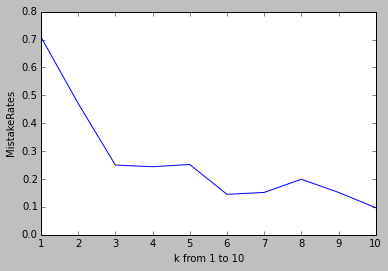
\includegraphics[width = 4.5in, keepaspectratio]{mrVsK.png}
\end{enumerate}

\subsection{Some useful functions}
No questions in this part.

\end{document}


